\documentclass[aspectratio=169,12pt]{beamer}
\usepackage[utf8]{inputenc}
\usepackage{amsmath, amssymb}
\usepackage{booktabs}
\usepackage{colortbl}
\usepackage{hyperref}
\usepackage{makecell}
\usepackage{ragged2e}
\usepackage{bytefield}
\usepackage{tikz}
\usetikzlibrary{arrows.meta, positioning, shapes.geometric, calc, tikzmark, shapes.misc}
\usepackage{tcolorbox}
\usetheme{Madrid}

\title{Computer Structure}
\subtitle{System}
\author{Lihu Rappoport}
\date{}

% Clock macro - draws a clock at given location
\newcommand{\drawclock}[1]{
    \begin{scope}[shift={(#1)}]
        \draw[thick] (0,0) circle (0.12);
        \draw[thick] (0,0) -- (0,0.08);
        \draw[thick] (0,0) -- (0.05,-0.03);
    \end{scope}
}

\begin{document}

\frame{\titlepage}

% Slide 1: Modern CPU Architecture Overview
\begin{frame}{Modern Multi-Core CPU Architecture}
\begin{columns}[T]
\column{0.55\textwidth}
\textbf{Hierarchy of Components:}
\begin{enumerate}
\item \textbf{Core}: Execution units + L1/L2 cache
\item \textbf{Socket/Package}: Multiple cores + shared L3 + memory controller
\item \textbf{System}: Multiple sockets + memory
\end{enumerate}

\vspace{0.3cm}
\textbf{Two Types of Interconnects:}
\begin{itemize}
\item \textcolor{blue}{\textbf{Intra-socket}}: Connects cores within CPU
\item \textcolor{red}{\textbf{Inter-socket}}: Connects different CPUs
\end{itemize}

\column{0.45\textwidth}
\begin{center}
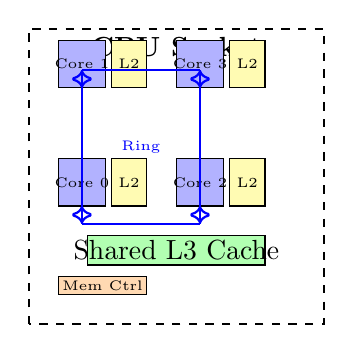
\begin{tikzpicture}[scale=0.75]
% Socket box
\draw[thick, dashed] (-0.5,-0.5) rectangle (4.5,4.5);
\node at (2,4.2) {\textbf{CPU Socket}};

% Cores
\foreach \x in {0,1} {
    \foreach \y in {0,1} {
        \pgfmathtruncatemacro{\cnum}{\x*2+\y}
        \draw[fill=blue!30] (\x*2,\y*2+1.5) rectangle (\x*2+0.8,\y*2+2.3);
        \node at (\x*2+0.4,\y*2+1.9) {\tiny Core \cnum};
        \draw[fill=yellow!30] (\x*2+0.9,\y*2+1.5) rectangle (\x*2+1.5,\y*2+2.3);
        \node at (\x*2+1.2,\y*2+1.9) {\tiny L2};
    }
}

% Shared L3
\draw[fill=green!30] (0.5,0.5) rectangle (3.5,1);
\node at (2,0.75) {Shared L3 Cache};

% Memory Controller
\draw[fill=orange!30] (0,0) rectangle (1.5,0.3);
\node at (0.75,0.15) {\tiny Mem Ctrl};

% Ring interconnect
\draw[thick, blue, <->] (0.4,1.5) -- (0.4,1.2);
\draw[thick, blue, <->] (2.4,1.5) -- (2.4,1.2);
\draw[thick, blue, <->] (0.4,3.5) -- (0.4,3.8);
\draw[thick, blue, <->] (2.4,3.5) -- (2.4,3.8);
\draw[thick, blue] (0.4,1.2) -- (2.4,1.2);
\draw[thick, blue] (0.4,3.8) -- (2.4,3.8);
\draw[thick, blue] (0.4,1.2) -- (0.4,3.8);
\draw[thick, blue] (2.4,1.2) -- (2.4,3.8);
\node[blue] at (1.4,2.5) {\tiny Ring};

\end{tikzpicture}
\end{center}
\end{columns}
\end{frame}

% Slide 2: Intra-Socket Interconnects
\begin{frame}{Intra-Socket Interconnects}
Connect cores, caches, memory controllers, and I/O within a single CPU package

\begin{center}
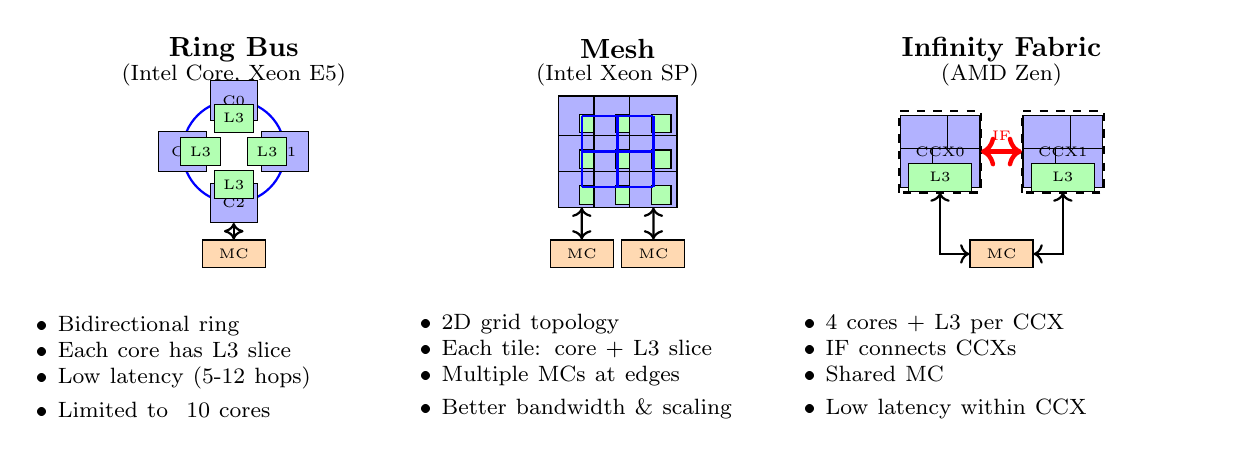
\begin{tikzpicture}[scale=0.65,
    core/.style={draw, rectangle, fill=blue!30, minimum width=0.6cm, minimum height=0.5cm},
    cache/.style={draw, rectangle, fill=green!30, minimum width=2.5cm, minimum height=0.3cm},
    mc/.style={draw, rectangle, fill=orange!30, minimum width=0.8cm, minimum height=0.3cm}
]

% Ring Topology
\begin{scope}[shift={(-5,0)}]
\node at (0, 2) {\textbf{Ring Bus}};
\node at (0, 1.5) {\footnotesize (Intel Core, Xeon E5)};
% Draw ring
\draw[thick, blue] (0,0) circle (1cm);
% Add components with L3 slices
\foreach \i/\angle in {0/90, 1/0, 2/270, 3/180} {
    \node[core] (c\i) at (\angle:1) {\tiny C\i};
    \node[cache, minimum width=0.3cm] at (\angle:0.65) {\tiny L3};
}
\node[mc] (ring_mc) at (0,-2) {\tiny MC};
\draw[<->, thick] (c2) -- (ring_mc.north);

% Annotations
\node[text width=5cm, align=left] at (0,-4.2) {
\footnotesize
• Bidirectional ring\\
• Each core has L3 slice\\
• Low latency (5-12 hops)\\
• Limited to ~10 cores
};
\end{scope}

% Mesh Topology
\begin{scope}[shift={(2.5,0)}]
\node at (0, 2) {\textbf{Mesh}};
\node at (0, 1.5) {\footnotesize (Intel Xeon SP)};
% Draw mesh with integrated L3
\foreach \x in {-1,0,1} {
    \foreach \y in {-1,0,1} {
        \node[core] (m\x\y) at (\x*0.7,\y*0.7) {\tiny};
        \node[cache, minimum width=0.25cm, minimum height=0.15cm] at (\x*0.7+0.15,\y*0.7-0.15) {\tiny};
    }
}
% Draw connections
\foreach \x in {-1,0,1} {
    \draw[blue, thick] (\x*0.7,-1*0.7) -- (\x*0.7,1*0.7);
}
\foreach \y in {-1,0,1} {
    \draw[blue, thick] (-1*0.7,\y*0.7) -- (1*0.7,\y*0.7);
}
\node[mc] (mesh_mc1) at (-0.7,-2) {\tiny MC};
\node[mc] (mesh_mc2) at (0.7,-2) {\tiny MC};
\draw[<->, thick] (m-1-1) -- (mesh_mc1.north);
\draw[<->, thick] (m1-1) -- (mesh_mc2.north);

% Annotations
\node[text width=5cm, align=left] at (0,-4.2) {
\footnotesize
• 2D grid topology\\
• Each tile: core + L3 slice\\
• Multiple MCs at edges\\
• Better bandwidth \& scaling
};
\end{scope}

% Crossbar/IF
\begin{scope}[shift={(10,0)}]
\node at (0, 2) {\textbf{Infinity Fabric}};
\node at (0, 1.5) {\footnotesize (AMD Zen)};

% CCX 0
\begin{scope}[shift={(-1.2,0)}]
\draw[dashed, thick] (-0.8,-0.8) rectangle (0.8,0.8);
\foreach \i in {0,1,2,3} {
    \node[core] (z0\i) at ({45+\i*90}:0.45) {\tiny};
}
\node[cache, minimum width=0.8cm, minimum height=0.2cm] at (0,-0.5) {\tiny L3};
\node at (0,0) {\tiny CCX0};
\end{scope}

% CCX 1
\begin{scope}[shift={(1.2,0)}]
\draw[dashed, thick] (-0.8,-0.8) rectangle (0.8,0.8);
\foreach \i in {0,1,2,3} {
    \node[core] (z1\i) at ({45+\i*90}:0.45) {\tiny};
}
\node[cache, minimum width=0.8cm, minimum height=0.2cm] at (0,-0.5) {\tiny L3};
\node at (0,0) {\tiny CCX1};
\end{scope}

% Infinity Fabric interconnect
\draw[<->, ultra thick, red] (-0.4,0) -- node[above, font=\tiny] {IF} (0.4,0);

% Memory controller
\node[mc] (ifmc) at (0,-2) {\tiny MC};
\draw[<->, thick] (-1.2,-0.8) |- (ifmc.west);
\draw[<->, thick] (1.2,-0.8) |- (ifmc.east);

% Annotations
\node[text width=5cm, align=left] at (0,-4.2) {
\footnotesize
• 4 cores + L3 per CCX\\
• IF connects CCXs\\
• Shared MC\\
• Low latency within CCX
};
\end{scope}

\end{tikzpicture}
\end{center}

All cores can access all cache and memory controllers, but with varying latency
\end{frame}

% Slide 3: Ring Interconnect Details
\begin{frame}{Ring Interconnect: How It Works}
\begin{columns}[T]
\column{0.5\textwidth}
\textbf{Ring Architecture:}
\begin{itemize}
\item Bidirectional rings (clockwise + counter-clockwise)
\item Each "stop" contains:
  \begin{itemize}
  \item CPU core
  \item L3 cache slice
  \item Connection logic
  \end{itemize}
\item Messages take shortest path
\item Typically 32-byte data ring
\end{itemize}

\vspace{0.3cm}
\textbf{Why Rings Work Well (up to a point):}
\begin{itemize}
\item Simple to implement
\item Predictable latency
\item Good bandwidth for small core counts
\item Power efficient
\end{itemize}

\column{0.5\textwidth}
\begin{center}
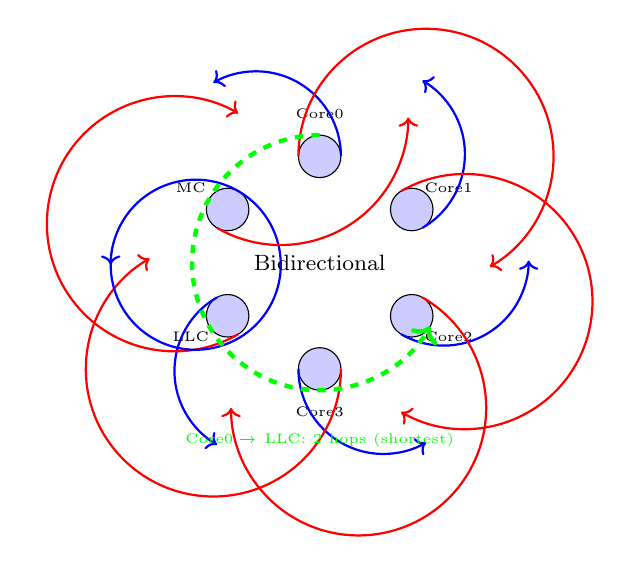
\begin{tikzpicture}[scale=0.9]
% Draw ring stops
\foreach \i/\name in {0/Core0, 1/Core1, 2/Core2, 3/Core3, 4/LLC, 5/MC} {
    \pgfmathsetmacro{\angle}{90-\i*60}
    \coordinate (stop\i) at (\angle:1.5);
    \draw[fill=blue!20] (\angle:1.5) circle (0.3);
    \node at (\angle:2.1) {\tiny \name};
}

% Draw ring connections
\foreach \i in {0,...,5} {
    \pgfmathtruncatemacro{\next}{mod(\i+1,6)}
    \pgfmathsetmacro{\angle}{90-\i*60}
    \pgfmathsetmacro{\nextangle}{90-\next*60}
    \draw[->, thick, blue] (\angle:1.5) ++({\angle-90}:0.3) arc ({\angle-90}:{\nextangle+90}:1.2);
    \draw[->, thick, red] (\angle:1.5) ++({\angle+90}:0.3) arc ({\angle+90}:{\nextangle-90}:1.8);
}

\node at (0,0) {\footnotesize Bidirectional};

% Example path
\draw[->, ultra thick, green, dashed] (90:1.8) arc (90:330:1.8);
\node[green] at (0,-2.5) {\tiny Core0 → LLC: 2 hops (shortest)};
\end{tikzpicture}
\end{center}

\textbf{Limitations:}
\begin{itemize}
\item Bandwidth shared by all stops
\item Latency grows with core count
\item Not suitable for >10-12 cores
\end{itemize}
\end{columns}
\end{frame}

% Slide 4: Inter-Socket Interconnects
\begin{frame}{Inter-Socket Interconnects}
\textbf{Connecting Multiple CPUs in a System}

\begin{center}
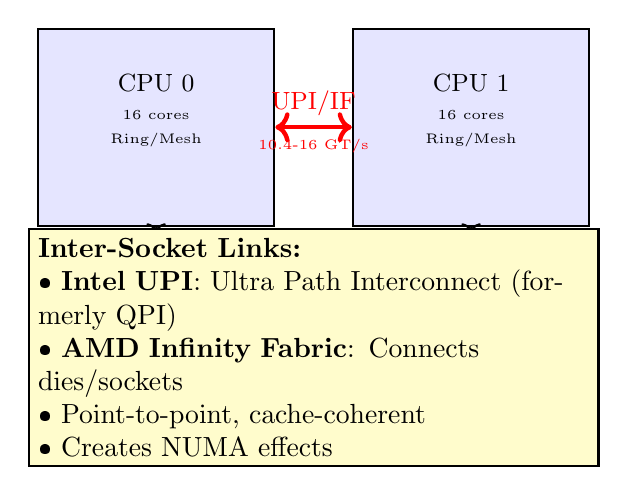
\begin{tikzpicture}[scale=0.8,
    socket/.style={draw, thick, fill=blue!10, minimum width=3cm, minimum height=2.5cm},
    memory/.style={draw, fill=gray!20, minimum width=2.5cm, minimum height=0.5cm}
]

% Two socket system
\node[socket] (cpu0) at (0,0) {};
\node at (0,0.7) {\small CPU 0};
\node at (0,0.2) {\tiny 16 cores};
\node at (0,-0.2) {\tiny Ring/Mesh};
\node[memory] (mem0) at (0,-2) {\small Memory 0};
\draw[<->, thick] (cpu0.south) -- (mem0.north);

\node[socket] (cpu1) at (5,0) {};
\node at (5,0.7) {\small CPU 1};
\node at (5,0.2) {\tiny 16 cores};
\node at (5,-0.2) {\tiny Ring/Mesh};
\node[memory] (mem1) at (5,-2) {\small Memory 1};
\draw[<->, thick] (cpu1.south) -- (mem1.north);

% Inter-socket link
\draw[<->, ultra thick, red] (cpu0.east) -- node[above] {\small UPI/IF} node[below] {\tiny 10.4-16 GT/s} (cpu1.west);

% Annotations
\node[draw, thick, fill=yellow!20, text width=7cm] at (2.5,-3.5) {
\textbf{Inter-Socket Links:}\\
• \textbf{Intel UPI}: Ultra Path Interconnect (formerly QPI)\\
• \textbf{AMD Infinity Fabric}: Connects dies/sockets\\
• Point-to-point, cache-coherent\\
• Creates NUMA effects
};

\end{tikzpicture}
\end{center}

\vspace{0.3cm}
\textbf{Performance Impact:}
\begin{columns}[T]
\column{0.5\textwidth}
\begin{itemize}
\item Local memory: \textasciitilde80-100 ns
\item Remote memory: \textasciitilde120-150 ns
\end{itemize}
\column{0.5\textwidth}
\begin{itemize}
\item Cross-socket bandwidth: 20-40 GB/s
\item Local memory bandwidth: 50-100 GB/s
\end{itemize}
\end{columns}
\end{frame}

% Slide 5: Complete System View
\begin{frame}{Complete System View: From Core to System}
\begin{center}
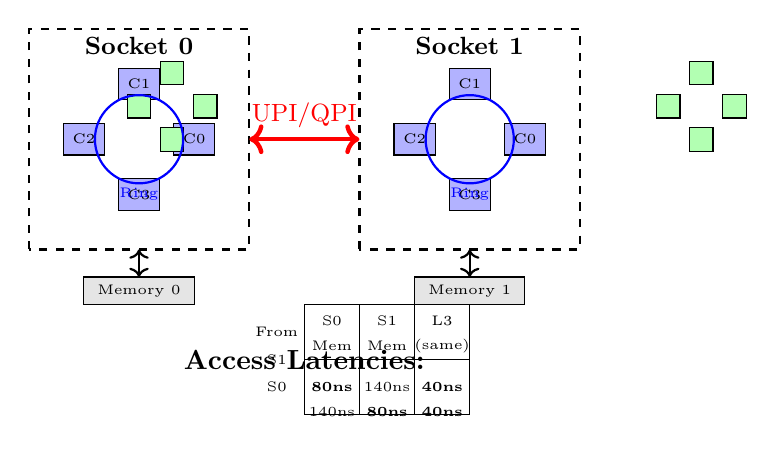
\begin{tikzpicture}[scale=0.7,
    core/.style={draw, fill=blue!30, minimum width=0.4cm, minimum height=0.4cm},
    l3/.style={draw, fill=green!30, minimum width=0.3cm, minimum height=0.3cm}
]

% Socket 0
\draw[thick, dashed] (-1,-1) rectangle (3,3);
\node at (1,2.7) {\small \textbf{Socket 0}};

% Cores with ring
\foreach \i in {0,1,2,3} {
    \pgfmathsetmacro{\x}{1+cos(\i*90)}
    \pgfmathsetmacro{\y}{1+sin(\i*90)}
    \node[core] at (\x,\y) {\tiny C\i};
    \node[l3] at (\x*0.6+1,\y*0.6+1) {};
}
\draw[blue, thick] (1,1) circle (0.8);
\node[blue] at (1,0) {\tiny Ring};

% Socket 1
\draw[thick, dashed] (5,-1) rectangle (9,3);
\node at (7,2.7) {\small \textbf{Socket 1}};

% Cores with ring
\foreach \i in {0,1,2,3} {
    \pgfmathsetmacro{\x}{7+cos(\i*90)}
    \pgfmathsetmacro{\y}{1+sin(\i*90)}
    \node[core] at (\x,\y) {\tiny C\i};
    \node[l3] at (\x*0.6+7,\y*0.6+1) {};
}
\draw[blue, thick] (7,1) circle (0.8);
\node[blue] at (7,0) {\tiny Ring};

% Memory
\draw[fill=gray!20] (0,-2) rectangle (2,-1.5) node[pos=.5] {\tiny Memory 0};
\draw[fill=gray!20] (6,-2) rectangle (8,-1.5) node[pos=.5] {\tiny Memory 1};

% Connections
\draw[<->, thick] (1,-1) -- (1,-1.5);
\draw[<->, thick] (7,-1) -- (7,-1.5);
\draw[<->, ultra thick, red] (3,1) -- node[above] {\small UPI/QPI} (5,1);

% Latency table
\node at (4,-3) {\textbf{Access Latencies:}};
\begin{scope}[shift={(4,-4)}]
\draw (0,0) grid (3,2);
\node at (-0.5,1.5) {\tiny From};
\node at (-0.5,0.5) {\tiny S0};
\node at (-0.5,1) {\tiny S1};
\node at (0.5,1.7) {\tiny S0};
\node at (1.5,1.7) {\tiny S1};
\node at (2.5,1.7) {\tiny L3};
\node at (0.5,1.25) {\tiny Mem};
\node at (1.5,1.25) {\tiny Mem};
\node at (2.5,1.25) {\tiny (same)};
\node at (0.5,0.5) {\textbf{\tiny 80ns}};
\node at (1.5,0.5) {\tiny 140ns};
\node at (2.5,0.5) {\textbf{\tiny 40ns}};
\node at (0.5,0.05) {\tiny 140ns};
\node at (1.5,0.05) {\textbf{\tiny 80ns}};
\node at (2.5,0.05) {\textbf{\tiny 40ns}};
\end{scope}

\end{tikzpicture}
\end{center}

\textbf{Key Insights:}
\begin{itemize}
\item Intra-socket communication (ring/mesh) is fast: 5-15 cycles
\item Inter-socket communication (UPI/IF) is slower: 50+ cycles  
\item Memory access hierarchy: L3 cache → Local DRAM → Remote DRAM
\item Software must be aware of this hierarchy for optimal performance
\end{itemize}
\end{frame}

% Slide 6: Software Implications
\begin{frame}{Software Implications}
\begin{columns}[T]
\column{0.5\textwidth}
\textbf{What Software Developers Need to Know:}

\vspace{0.2cm}
\textbf{1. Cache Coherency}
\begin{itemize}
\item Maintained automatically
\item But costs performance
\item Worse across sockets
\end{itemize}

\vspace{0.2cm}
\textbf{2. Memory Allocation}
\begin{itemize}
\item First-touch policy
\item NUMA-aware allocation
\item Thread-local storage
\end{itemize}

\vspace{0.2cm}
\textbf{3. Thread Placement}
\begin{itemize}
\item Pin threads to cores
\item Keep related threads on same socket
\item Minimize cross-socket communication
\end{itemize}

\column{0.5\textwidth}
\textbf{Performance Tips:}

\begin{enumerate}
\item \textbf{Check your topology:}\\
   \texttt{lscpu -e} or \texttt{lstopo}
   
\item \textbf{Quick improvement:}\\
   \texttt{numactl --cpunodebind=0 ./app}
   
\item \textbf{For shared data:}\\
   Place on socket with most accessors
   
\item \textbf{For partitioned data:}\\
   Align partitions to NUMA nodes
\end{enumerate}

\vspace{0.3cm}
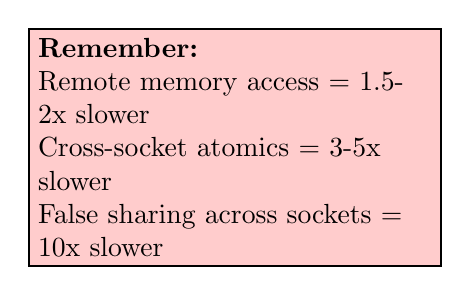
\begin{tikzpicture}
\node[draw, thick, fill=red!20, text width=5cm] at (0,0) {
\textbf{Remember:}\\
Remote memory access = 1.5-2x slower\\
Cross-socket atomics = 3-5x slower\\
False sharing across sockets = 10x slower
};
\end{tikzpicture}
\end{columns}
\end{frame}


% Slide 1: Introduction to NUMA
\begin{frame}{From UMA to NUMA}
\begin{columns}[T]
\column{0.48\textwidth}
\textbf{Uniform Memory Access (UMA)}
\begin{itemize}
\item All cores share single memory controller
\item Equal latency to all memory
\item Simple programming model
\item \textcolor{red}{Bottleneck}: Memory controller bandwidth
\end{itemize}

\column{0.52\textwidth}
\textbf{Non-Uniform Memory Access (NUMA)}
\begin{itemize}
\item Multiple memory controllers
\item Memory "local" to each CPU socket
\item Variable memory latency
\item Higher aggregate bandwidth
\item \textcolor{orange}{Challenge}: Data locality matters!
\end{itemize}
\end{columns}

\vspace{0.3cm}
\begin{center}
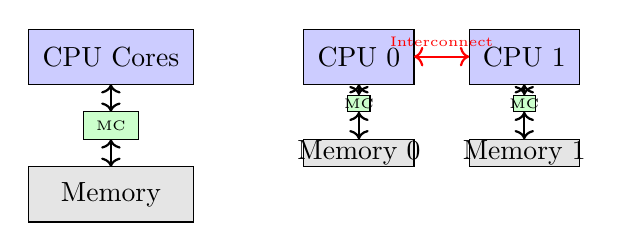
\begin{tikzpicture}[scale=0.7]
% UMA diagram
\draw[fill=blue!20] (-5.5,0) rectangle (-2.5,1) node[pos=.5] {CPU Cores};
\draw[fill=green!20] (-4.5,-1) rectangle (-3.5,-0.5) node[pos=.5, font=\tiny] {MC};
\draw[fill=gray!20] (-5.5,-2.5) rectangle (-2.5,-1.5) node[pos=.5] {Memory};
\draw[<->, thick] (-4,0) -- (-4,-0.5);
\draw[<->, thick] (-4,-1) -- (-4,-1.5);

% NUMA diagram
% Node 0
\draw[fill=blue!20] (-0.5,0) rectangle (1.5,1) node[pos=.5] {CPU 0};
\draw[fill=green!20] (0.3,-0.5) rectangle (0.7,-0.2) node[pos=.5, font=\tiny] {MC};
\draw[fill=gray!20] (-0.5,-1.5) rectangle (1.5,-1) node[pos=.5] {Memory 0};
\draw[<->, thick] (0.5,0) -- (0.5,-0.2);
\draw[<->, thick] (0.5,-0.5) -- (0.5,-1);

% Node 1
\draw[fill=blue!20] (2.5,0) rectangle (4.5,1) node[pos=.5] {CPU 1};
\draw[fill=green!20] (3.3,-0.5) rectangle (3.7,-0.2) node[pos=.5, font=\tiny] {MC};
\draw[fill=gray!20] (2.5,-1.5) rectangle (4.5,-1) node[pos=.5] {Memory 1};
\draw[<->, thick] (3.5,0) -- (3.5,-0.2);
\draw[<->, thick] (3.5,-0.5) -- (3.5,-1);

% Interconnect
\draw[<->, thick, red] (1.5,0.5) -- node[above, font=\tiny] {Interconnect} (2.5,0.5);
\end{tikzpicture}
\end{center}
\end{frame}

% Slide 2: NUMA Topology
\begin{frame}{NUMA Node Topology}
\begin{columns}[T]
\column{0.45\textwidth}
\textbf{Key Concepts:}
\begin{itemize}
\item \textbf{NUMA Node}: CPU cores + local memory
\item \textbf{Socket}: Physical CPU package
\item \textbf{Distance}: Relative memory access cost
\item \textbf{Affinity}: Binding threads/memory to nodes
\end{itemize}

\vspace{0.3cm}
\textbf{Typical 2-Socket System:}
\begin{itemize}
\item Local memory: \textasciitilde100 cycles
\item Remote memory: \textasciitilde150-200 cycles
\item Can be 50-100\% slower!
\end{itemize}

\column{0.55\textwidth}
\begin{center}
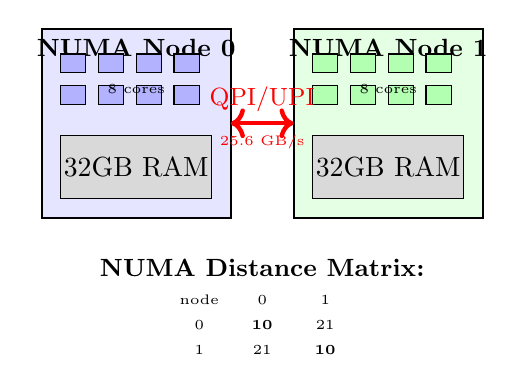
\begin{tikzpicture}[scale=0.8]
% NUMA Node 0
\draw[thick, fill=blue!10] (0,0) rectangle (3,3);
\node at (1.5, 2.7) {\small \textbf{NUMA Node 0}};
\foreach \x in {0.3,0.9,1.5,2.1} {
    \foreach \y in {1.8,2.3} {
        \draw[fill=blue!30] (\x,\y) rectangle (\x+0.4,\y+0.3);
    }
}
\node at (1.5, 2.05) {\tiny 8 cores};
\draw[fill=gray!30] (0.3,0.3) rectangle (2.7,1.3);
\node at (1.5,0.8) {32GB RAM};

% NUMA Node 1
\draw[thick, fill=green!10] (4,0) rectangle (7,3);
\node at (5.5, 2.7) {\small \textbf{NUMA Node 1}};
\foreach \x in {4.3,4.9,5.5,6.1} {
    \foreach \y in {1.8,2.3} {
        \draw[fill=green!30] (\x,\y) rectangle (\x+0.4,\y+0.3);
    }
}
\node at (5.5, 2.05) {\tiny 8 cores};
\draw[fill=gray!30] (4.3,0.3) rectangle (6.7,1.3);
\node at (5.5,0.8) {32GB RAM};

% Interconnect
\draw[<->, ultra thick, red] (3,1.5) -- node[above] {\small QPI/UPI} node[below] {\tiny 25.6 GB/s} (4,1.5);

% Distance matrix
\node at (3.5, -0.8) {\small \textbf{NUMA Distance Matrix:}};
\node at (2.5, -1.3) {\tiny node};
\node at (3.5, -1.3) {\tiny 0};
\node at (4.5, -1.3) {\tiny 1};
\node at (2.5, -1.7) {\tiny 0};
\node at (3.5, -1.7) {\tiny \textbf{10}};
\node at (4.5, -1.7) {\tiny 21};
\node at (2.5, -2.1) {\tiny 1};
\node at (3.5, -2.1) {\tiny 21};
\node at (4.5, -2.1) {\tiny \textbf{10}};
\end{tikzpicture}
\end{center}
\end{columns}
\end{frame}

% Slide 3: Interconnect Topologies
\begin{frame}{Interconnect Topologies}
\begin{center}
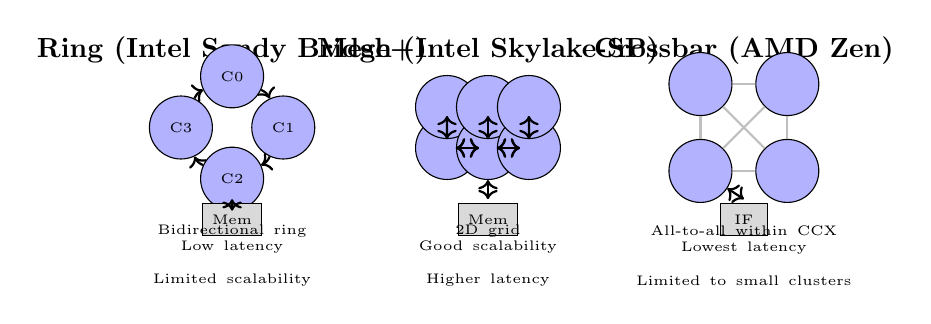
\begin{tikzpicture}[scale=0.65,
    cpu/.style={draw, circle, fill=blue!30, minimum size=0.8cm},
    mem/.style={draw, rectangle, fill=gray!30, minimum width=0.6cm, minimum height=0.4cm}
]

% Ring (Intel)
\begin{scope}[shift={(0,0)}]
\node at (0, 1.5) {\textbf{Ring (Intel Sandy Bridge+)}};
\foreach \i in {0,1,2,3} {
    \node[cpu] (c\i) at ({90-\i*90}:1) {\tiny C\i};
}
\foreach \i in {0,1,2,3} {
    \pgfmathtruncatemacro{\j}{mod(\i+1,4)}
    \draw[->, thick] (c\i) to[bend left=20] (c\j);
}
\node[mem] at (0,-1.8) {\tiny Mem};
\draw[<->, thick] (c2) -- (0,-1.4);
\node[text width=3cm, align=center] at (0,-2.5) {\tiny Bidirectional ring\\ Low latency\\ Limited scalability};
\end{scope}

% Mesh (Intel)
\begin{scope}[shift={(5,0)}]
\node at (0, 1.5) {\textbf{Mesh (Intel Skylake-SP)}};
\foreach \x in {0,1,2} {
    \foreach \y in {0,1} {
        \node[cpu] (m\x\y) at (\x*0.8-0.8,\y*0.8-0.4) {\tiny};
    }
}
% Horizontal connections
\foreach \y in {0,1} {
    \draw[<->, thick] (m00) -- (m10);
    \draw[<->, thick] (m10) -- (m20);
}
% Vertical connections
\foreach \x in {0,1,2} {
    \draw[<->, thick] (m\x0) -- (m\x1);
}
\node[mem] at (0,-1.8) {\tiny Mem};
\draw[<->, thick] (m10) -- (0,-1.4);
\node[text width=3cm, align=center] at (0,-2.5) {\tiny 2D grid\\ Good scalability\\ Higher latency};
\end{scope}

% Crossbar (AMD)
\begin{scope}[shift={(10,0)}]
\node at (0, 1.5) {\textbf{Crossbar (AMD Zen)}};
\foreach \i in {0,1,2,3} {
    \node[cpu] (x\i) at ({45+\i*90}:1.2) {\tiny};
}
% Full crossbar connections
\foreach \i in {0,1,2} {
    \foreach \j in {1,2,3} {
        \ifnum\i<\j
            \draw[-, thick, gray!50] (x\i) -- (x\j);
        \fi
    }
}
\node[mem] at (0,-1.8) {\tiny IF};
\draw[<->, thick] (x2) -- (0,-1.4);
\node[text width=3cm, align=center] at (0,-2.5) {\tiny All-to-all within CCX\\ Lowest latency\\ Limited to small clusters};
\end{scope}

\end{tikzpicture}
\end{center}

\vspace{0.3cm}
\textbf{Software Impact:}
\begin{itemize}
\item Different topologies $\rightarrow$ different performance characteristics
\item Ring: predictable latency, but can saturate with many cores
\item Mesh: better for many-core scaling, but more variable latency
\item Crossbar: excellent for small core counts, used in AMD's CCX design
\end{itemize}
\end{frame}

% Slide 4: Software Implications
\begin{frame}{NUMA: Software Implications}
\begin{columns}[T]
\column{0.5\textwidth}
\textbf{Performance Impact:}
\begin{itemize}
\item Remote memory access: 50-100\% slower
\item Cache coherency traffic across nodes
\item Memory bandwidth per node is limited
\item False sharing amplified across NUMA
\end{itemize}

\vspace{0.3cm}
\textbf{Common Issues:}
\begin{itemize}
\item Thread migration between nodes
\item Data allocated on "wrong" node
\item Unbalanced memory usage
\item Lock contention across nodes
\end{itemize}

\column{0.5\textwidth}
\textbf{Best Practices:}
\begin{enumerate}
\item \textbf{First-touch policy}: Allocate memory on the node that first accesses it
\item \textbf{Thread affinity}: Pin threads to specific cores/nodes
\item \textbf{Data partitioning}: Align data structures to NUMA boundaries
\item \textbf{NUMA-aware allocation}: Use \texttt{numa\_alloc\_onnode()}
\end{enumerate}

\vspace{0.3cm}
\textbf{Tools:}
\begin{itemize}
\item \texttt{numactl}: Control NUMA policy
\item \texttt{lstopo}: Visualize topology
\item \texttt{numastat}: Memory statistics
\item \texttt{perf}: Profile NUMA events
\end{itemize}
\end{columns}
\end{frame}

% Slide 5: NUMA Code Example
\begin{frame}[fragile]{NUMA-Aware Programming Example}
\begin{columns}[T]
\column{0.5\textwidth}
\textbf{NUMA-Unaware Code:}
\begin{tcolorbox}[colback=red!5!white, colframe=red!50!black, boxrule=0.5pt, left=1pt, right=1pt, top=1pt, bottom=1pt]
{\scriptsize
\begin{verbatim}
// Thread 0 allocates all data
float* data = malloc(N * sizeof(float));

// All threads access same array
#pragma omp parallel
{
  int tid = omp_get_thread_num();
  int chunk = N / num_threads;
  int start = tid * chunk;
  
  // Remote memory access!
  for(int i = start; i < start+chunk; i++)
    data[i] = compute(i);
}
\end{verbatim}
}
\end{tcolorbox}

\column{0.5\textwidth}
\textbf{NUMA-Aware Code:}
\begin{tcolorbox}[colback=green!5!white, colframe=green!50!black, boxrule=0.5pt, left=1pt, right=1pt, top=1pt, bottom=1pt]
{\scriptsize
\begin{verbatim}
#pragma omp parallel
{
  int tid = omp_get_thread_num();
  int chunk = N / num_threads;
  
  // Each thread allocates locally
  float* local_data = 
    numa_alloc_local(chunk * sizeof(float));
  
  // Access local memory only
  for(int i = 0; i < chunk; i++)
    local_data[i] = compute(tid*chunk + i);
    
  // Copy to global if needed
  memcpy(&data[tid*chunk], local_data, ...);
}
\end{verbatim}
}
\end{tcolorbox}
\end{columns}

\vspace{0.3cm}
\textbf{Performance difference can be 2-3x for memory-bound workloads!}
\end{frame}

% Slide 6: Practical NUMA Considerations
\begin{frame}{Practical NUMA Considerations}
\begin{columns}[T]
\column{0.55\textwidth}
\textbf{When NUMA Matters Most:}
\begin{itemize}
\item Large working sets (> L3 cache)
\item Memory-bandwidth intensive apps
\item Multi-socket servers
\item Database systems
\item Scientific computing (HPC)
\item In-memory key-value stores
\end{itemize}

\vspace{0.3cm}
\textbf{Quick Checks:}
\begin{itemize}
\item \texttt{lscpu | grep NUMA} - see topology
\item \texttt{numactl --hardware} - detailed info
\item \texttt{likwid-topology} - visual layout
\end{itemize}

\column{0.45\textwidth}
\begin{center}
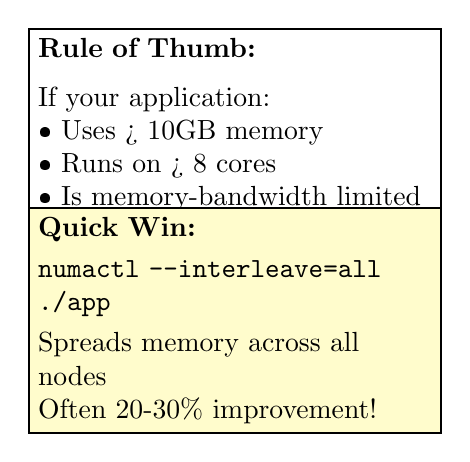
\begin{tikzpicture}[scale=0.8]
\node[text width=5cm, draw, thick] at (0,0) {
\textbf{Rule of Thumb:}\\[0.2cm]
If your application:\\
• Uses > 10GB memory\\
• Runs on > 8 cores\\
• Is memory-bandwidth limited\\[0.2cm]
$\Rightarrow$ \textcolor{red}{Consider NUMA optimization}
};

\node[text width=5cm, draw, thick, fill=yellow!20] at (0,-2.5) {
\textbf{Quick Win:}\\[0.1cm]
\texttt{numactl --interleave=all ./app}\\[0.1cm]
Spreads memory across all nodes\\
Often 20-30\% improvement!
};
\end{tikzpicture}
\end{center}
\end{columns}

\vspace{0.3cm}
\textbf{Modern Developments:}
\begin{itemize}
\item AMD Zen: Multiple NUMA nodes per socket (CCX/CCD design)
\item Intel Sub-NUMA Clustering (SNC): Divides socket into NUMA nodes
\item CXL: Enables memory pooling across systems
\end{itemize}
\end{frame}


\begin{frame}{Basic DRAM chip}
\textbf{DRAM:} 2D array of memory cells
\vspace{-0.2cm}

\begin{center}
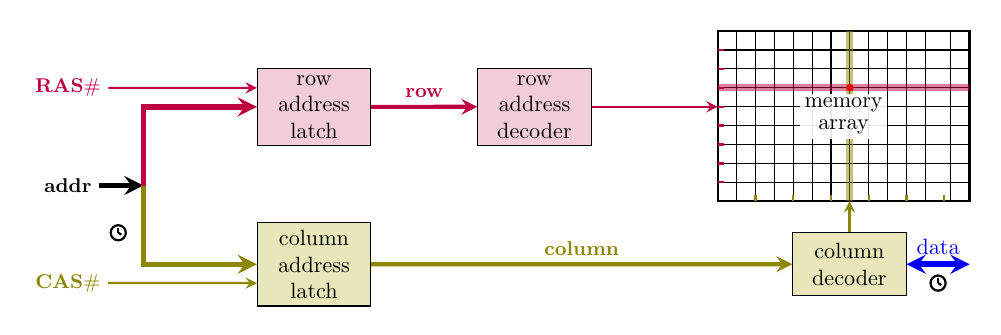
\begin{tikzpicture}[scale=0.8, transform shape,
    block/.style={draw, minimum width=1.8cm, minimum height=1cm, align=center},
    decoder/.style={draw, minimum width=1.8cm, minimum height=1.2cm, align=center},
    signal/.style={->, >=stealth, thick},
    label/.style={font=\small\bfseries}
]

% Origin point - move this to shift entire diagram
\coordinate (origin) at (0,25);

% Row Address Latch - positioned relative to origin
\node[block, text width=1.5cm, fill=purple!20] (rowlatch) at (origin) {row address latch};

% Column Address Latch - positioned relative to row latch
\node[block, text width=1.5cm, fill=olive!20] (collatch) at ([yshift=-2.5cm]rowlatch) {column address latch};

% Row Address decoder - positioned relative to row latch
\node[decoder, text width=1.5cm, fill=purple!20] (rowdecoder) at ([xshift=3.5cm]rowlatch) {row address decoder};

% Column decoder - positioned relative to column latch
\node[block, text width=1.5cm, fill=olive!20] (coldecoder) at ([xshift=8.5cm]collatch) {column decoder};

% Memory array - positioned relative to decoders
\coordinate (array_corner) at ([xshift=2cm, yshift=1.2cm]rowdecoder.east);
\draw[thick] (array_corner) rectangle ([xshift=4cm, yshift=-2.7cm]array_corner);
\foreach \x in {0.3,0.6,0.9,1.2,1.5,1.8,2.1,2.4,2.7,3,3.3,3.7} {
    \draw ([xshift=\x cm]array_corner) -- ([xshift=\x cm, yshift=-2.7cm]array_corner);
}
\foreach \y in {-0.3,-0.6,-0.9,-1.2,-1.5,-1.8,-2.1,-2.4} {
    \draw ([yshift=\y cm]array_corner) -- ([xshift=4cm, yshift=\y cm]array_corner);
}

% Input signals - positioned relative to latches
\node[label, purple] (ras) at ([xshift=-3cm, yshift=0.3cm]rowlatch.west) {RAS$\#$};
\draw[signal, purple] (ras) -- (ras -| rowlatch.west);

\node[label, olive] (cas) at ([xshift=-3cm, yshift=-0.3cm]collatch.west) {CAS$\#$};
\draw[signal, olive] (cas) -- (cas -| collatch.west);

% Address in the middle between the two latches
\node[label] (addr) at ($(rowlatch.west)!0.5!(collatch.west) + (-3,0)$) {addr};
\coordinate (addr_split) at ($(rowlatch.west)!0.5!(collatch.west) + (-1.8,0)$);

\draw[signal, line width=2pt] (addr.east) -- (addr_split);
% Branch to row and column latches
\draw[signal, purple, line width=2pt] (addr_split) -- (addr_split |- rowlatch.west) -- (rowlatch.west);
\draw[signal, olive, line width=2pt] (addr_split) -- (addr_split |- collatch.west) -- (collatch.west);

% Clock symbol relative to addr_split
\drawclock{$(addr_split) + (-0.4,-0.75)$}

% Connections between blocks
\draw[signal, purple, line width=1.5pt] (rowlatch.east) -- node[above, font=\small\bfseries, purple] {row} (rowdecoder.west);
\draw[signal, olive, line width=1.5pt] (collatch.east) -- node[above, font=\small\bfseries, olive] {column} (coldecoder.west);

% Row decoder to memory array with highlighted row
\draw[signal, purple] (rowdecoder.east) -- (rowdecoder.east -| array_corner);
% Draw wordlines and highlight one
\foreach \y in {-0.3,-0.6,-0.9,-1.2,-1.5,-1.8,-2.1,-2.4} {
    \draw[purple, thick] ([yshift=\y cm]array_corner) -- ++(0.1,0);
}
% Highlight one row
\draw[purple, line width=2.5pt, opacity=0.5] ([yshift=-0.9cm]array_corner) -- ([xshift=4cm, yshift=-0.9cm]array_corner);

% Column decoder to memory array with highlighted column
\coordinate (array_bottom) at ([yshift=-2.7cm]array_corner);
\draw[signal, olive] (coldecoder.north) -- (coldecoder.north |- array_bottom);
% Draw bitlines and highlight one
\foreach \x in {0.6,1.2,1.8,2.4,3,3.6} {
    \draw[olive, thick] ([xshift=\x cm, yshift=-2.7cm]array_corner) -- ++(0,0.1);
}
% Highlight one column
\draw[olive, line width=2.5pt, opacity=0.5] ([xshift=2.1cm]array_corner) -- ([xshift=2.1cm, yshift=-2.7cm]array_corner);

% Mark intersection
\fill[red] ([xshift=2.1cm, yshift=-0.9cm]array_corner) circle (0.06);

% Data I/O - horizontal arrow
\draw[signal, blue, line width=2pt, <->] 
  (coldecoder.east) 
    -- node[midway, above, blue]{data} 
  ++(1,0);

% Clock symbol near data - relative to coldecoder
\drawclock{$(coldecoder.east) + (0.5,-0.3)$}

\node[
  align=center, 
  fill=white, 
  fill opacity=0.9,   % background 50% transparent
  text opacity=1,     % text fully visible
  inner sep=2pt
] at ([xshift=2cm, yshift=-1.35cm]array_corner) {memory\\[-2]array};

\end{tikzpicture}
\end{center}

\vspace{-0.2cm}
\textbf{DRAM access sequence:}
\begin{enumerate}
\item Row address on bus → Assert RAS$\#$ to latch row
\item Column address on bus → Assert CAS$\#$ to latch column (after t$_{RCD}$ delay)
\item Data available after CAS latency (CL)
\end{enumerate}

\end{frame}
\end{document}